
\documentclass{llncs}
\usepackage{llncsdoc}
\usepackage{graphicx} 
\usepackage{amsmath} 
\usepackage{caption}
\usepackage{url}
\usepackage{algorithmic}
\usepackage{listings}
\usepackage{makeidx}
\usepackage{enumitem}
\usepackage{subfig}

%
\begin{document}

\lstset{numbers=left, basicstyle=\small, numbersep=5pt, numberstyle=\tiny}

\tableofcontents

\section{rSLA DSL Introduction}
How can rSLA become the dominant language in the market (not standard). 

This document describes the structure, vocabulary and grammar (production rules) of the rSLA DSL. rSLA stands for ruby SLA and is implemented as a domain specific language (DSL) for the definition and management of service level agreements (SLAs) for cloud service provisioning. The language consists of the rSLA runtime that processes rSLA instances in a cloud environment like IBM Bluemix, of the rSLA editing environment and of Java xLets for monitoring and scheduling existing as well as new rSLA instances. 

rSLA accommodates the WSLA specification \cite{wsla} in the cloud setting. rSLA provides a concrete computing framework for the definition and management of cloud SLAs. The DSL uses Ruby code blocks, i.e. anonymous functions, to express SLA data and to describe their operations and functionality in an SLA runtime environment. Ruby blocks are perceived as closures that allow for customized definition of SLA properties, for their nesting with other rSLA components and their flexible handling in the program flow. 

The following sections specify the semantic significance of each object in the rSLA language, their logical definition, relationships to other objects and production rules for SLA formation and management.

\section{WSLA motivation}
rSLA is motivated by the WSLA specification \cite{wsla}, whose data structure is depicted in Figure \ref{wsla}. The WSLA specification defined the SLA structure for web services that are provisioned over distributed computing settings. The specification was originally implemented with the Java programming language and signified the state-of-the-art for numerous research efforts in the grid and utility computing domains. WSLA used the XML standard \cite{xml} to define and express SLA language concepts and grammar. First order logic was used to describe production rules and relational dependencies of inclusive elements.

The DSL inherits language concepts from WSLA. Figure \ref{rSLA} illustrates primary components of the rSLA language and their cardinality with respect to an SLA instance. 

%\begin{figure}
%        
%        \subfloat[subfigure 1\label{wsla}]
%               { 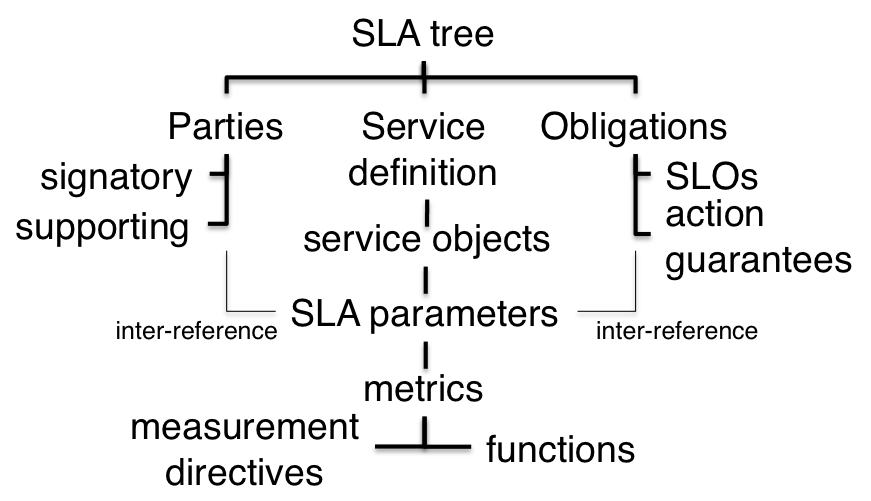
\includegraphics[width=\textwidth]{wsla}}
%    			\caption{WSLA skeleton structure}
%               \label{wsla}
%        \hfill
%        ~ %add desired spacing between images, e. g. ~, \quad, \qquad, \hfill etc.
%          %(or a blank line to force the subfigure onto a new line)
%        \subfloat[subfigure 2 \label{rsla}]{
%                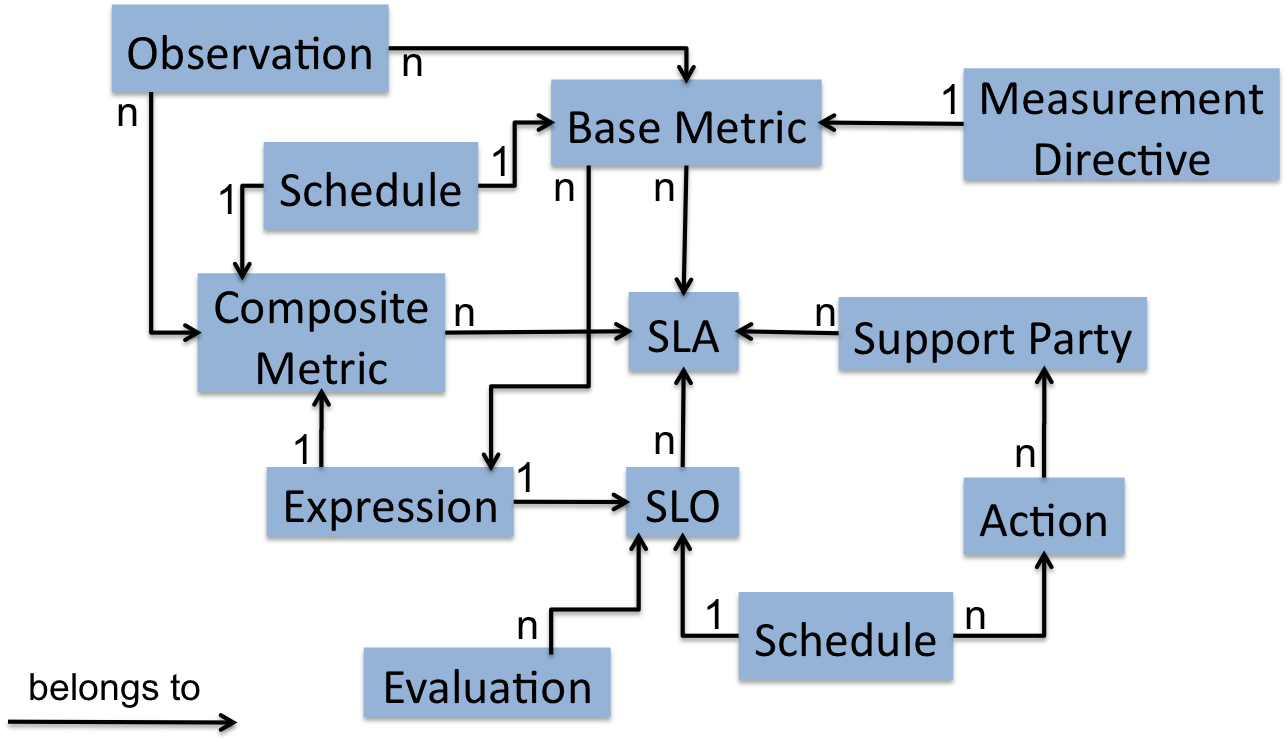
\includegraphics[width=\textwidth]{rSLA}
%                \caption{rSLA primary objects}
%                \label{rSLA}
%       
%        \caption{Figure \ref{wsla} illustrates the WSLA tree data structure \cite{wsla}. Figure \ref{rSLA} depicts inclusive relationships and cardinality of language elements for a single SLA object in the rSLA language.}\label{specs}
%\end{figure}

According to the WSLA specification \cite{wsla}, an SLA consists of three primary sections:
\begin{enumerate}
\item parties that specify the two signatory parties (customer - provider) and any support parties for the service execution,
\item service description or definition that specifies the agreed service context in terms of defined SLA parameters and metrics,
\item obligations or service level guarantees that define agreed responsibilities and promises with respect to service level values for all involved parties.
\end{enumerate}

The pilot version of the rSLA language is currently deployed as a ruby sinatra web service and tested on the IBM Bluemix cloud platform.

\section{rSLA BNF }

 %\cite{sidney}: get cfg, tuple, definitions
 A BNF language helps to formally describe the syntax of a programming language. The text describes grammars for the rSLA DSL using Backus-Naur form notation. An rSLA grammar can be extended to run as CFG (context-free grammar), which is helpful with writing new programming language rules.

In the rSLA BNF definition, every grammar rule is decomposed into another set of rules and/or literals. Non-terminal symbols are denoted as $<non-terminal-symbol>$ and the $::=$ symbol is translated as "expanded to" or "replaced with". In the text, terminal symbols or literals are denoted as 'literal'. 

\begin{lstlisting}[breaklines, firstnumber=auto, caption=rSLA BNF grammar rules]
grammarRule $::= <rule>+ 'literal' | <rule>$ ; 
"|" ::= choice, logical OR
";" ::= end of rule
"::=" ::= defined as/consists of
"?" ::= suffix to denote optional
"()" ::= denote grouping of rules and/or literals    
Kleene star * for 0 or more
Kleene plus + for 1 or more
".." ::= range
<digit> ::= '0'..'9'
<dow>   ::= 'a'..'z'
<number>  ::= <digit+> | <dow+>
<Id> ::= 'literal'| ('a'..'z'|'A'..'Z'|_|'0'..'9')* ;
<dateTime> ::= see ISO 8601 date time format
<string> ::= """<Unicode content>"""
<Unicode content> ::= See http://www.unicode.org/versions/Unicode7.0.0/
<URI> ::= See RFC 3986 (http://www.ietf.org/rfc/rfc3986.txt)
\end{lstlisting}

\subsection{rSLA vocabulary}
The rSLA language inherits from the WSLA specification \cite{wsla} the semantic decomposition of an SLA into a hierarchical tree, where the root node represents an SLA object. Nodes attached to the root denote SLA branches (e.g. base and composite metrics, service level objectives). 
\begin{figure}
  \centering
    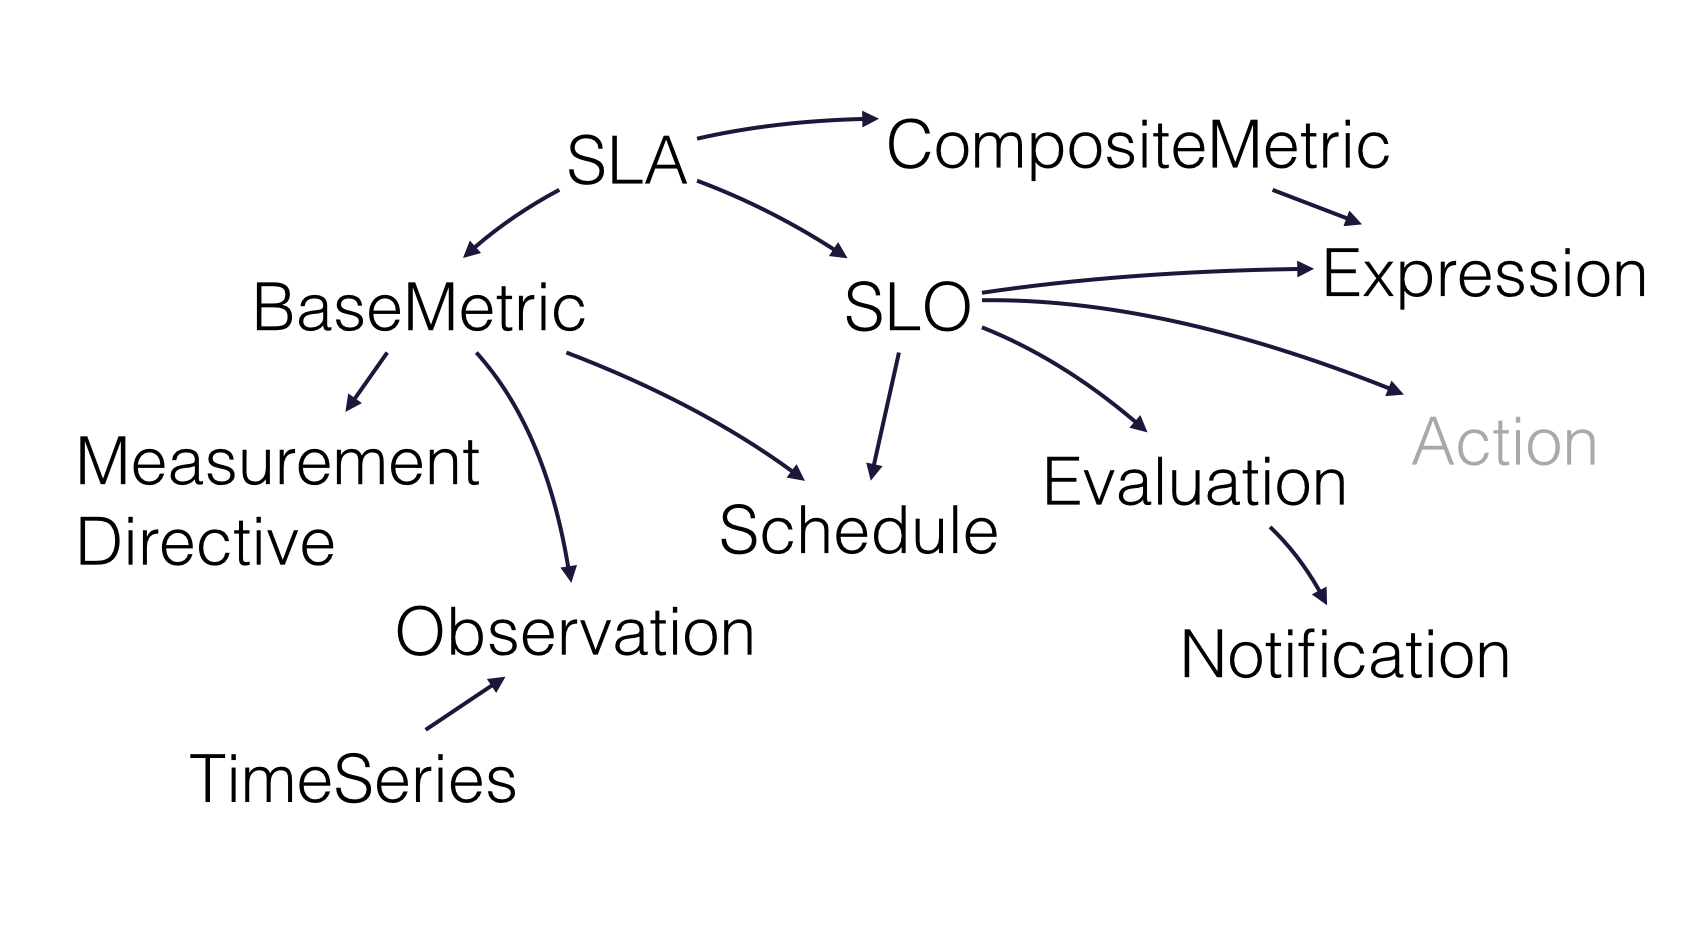
\includegraphics[width=0.5\textwidth]{rslauser}
    \caption{rSLA DSL user input diagram}
    \label{rSLA_diag}
\end{figure}
Figure \ref{rSLA_diag} illustrates a class diagram of the core rSLA DSL alphabet. Solid black arrows in Figure \ref{rSLA_diag} indicate that user-input is required to create the equivalent objects in an rSLA running environment. The alphabet is illustrated as a tree, where connections between nodes highlight relationships and nesting of SLA context. 

The rSLA alphabet consists of language elements that require user input for their creation in an rSLA runtime environment. A DSL user can directly edit code-block scripts in ruby, start a cloud rSLA service and create an active SLA object. 

In Figure \ref{rSLA_diag} language elements that require user-input represent tree branches for the creation of service level agreements. DSL user-input requires editing a ruby script to describe the attributes for any new rSLA object. The structure of such script is discussed in the following paragraphs as it is intepreted by the rSLA engine.

The rSLA language also contains elements, whose definition with an rSLA service requires that at least one SLA object exists (ex. base metric, slo). A DSL user can edit the context of such elements and associate them with required objects using code blocks in ruby SLA scripts.

\subsection{SLA object}\label{slaobject}

rSLA enables the generation and processing of SLA instances in a cloud runtime environment, where an rSLA service is deployed and running. The grammar excerpt in BNF notation illustrates the rSLA language rules for producing SLA objects:
%here need to add rule on the relationship between SLA and other objects
%an SLA contains all other objects OR the objects belong to an SLA? 
\begin{lstlisting}[breaklines, firstnumber=auto, caption=$<SLA>$ BNF grammar]
  <SLA> ::= (<baseMetric+>) (<compositeMetric*>)(<SLO+>) <customer> <provider> <description> <agreedTime>;
<description> ::= 'literal';
<customer> ::= 'literal';
<provider> ::= 'literal';
<agreedTime> ::= 'date-time literal';
\end{lstlisting}
rSLA exposes SLA information through ruby programming blocks that are simple to edit and process.
The rSLA DSL provides an SLA class for the generation of SLA objects that conform to attributes of ruby blocks as the following:
\begin{lstlisting}[caption=rSLA SLA definition, label=SLAlst]
sla do
  	tenant "XYZ Inc." 
  	provider "IBM"
  	description "This is a sample SLA"
  	creationTime "2015-01-30"
end 
\end{lstlisting}

An SLA object is defined by a description, an id and contains a date identifier to timestamp an object's creation time. A generated SLA is related to a single provider and a single customer, which are referenced by their unique ids. Additionally, an SLA is associated with:
\begin{itemize}[noitemsep,nolistsep]
\item 1 or more baseMetrics (section \ref{basemetric}), 
\item 0 or more compositeMetrics (section \ref{composite}) and
\item 1 or more SLOs (section \ref{slos}).
\end{itemize}  

The illustrated block provides information to the rSLA runtime environment regarding contracting entities, i.e. service customer and provider. rSLA defines a single customer and a single provider rule for every SLA object \cite{wsla}. A DSL user can set the identity of respective parties through such properties and also extend them to reflect domain specific needs.

Every new SLA object is identified by a unique id. The SLA identifier is used by the rSLA runtime to index an SLA object into available persistence middlewares and to associate it with related objects in the runtime environment. 

\subsection{Base metric}\label{basemetric}
A base metric inherits the semantics of resource metrics by the WSLA specification \cite{wsla} and adjusts their meaning into the cloud setting. The rSLA language implements a simple BNF grammar for the definition of $baseMetric$ objects:
\begin{lstlisting}[breaklines, firstnumber=auto, caption=$<BaseMetric>$ BNF grammar]
<baseMetric> ::=  <name> <type> <source> <unit> <measurementDirective> <schedule+> ;
<name> ::= 'literal';<string>
<type> 
<source> 
<unit>
<measurementDirective> ::= <measurementDirective>;
<schedule> ::= <schedule>;
\end{lstlisting}

The rSLA DSL implements the $<baseMetric>$ grammar into a class that generates $baseMetric$ objects in an rSLA runtime environment. A base metric represents a service metric that is used by one or more SLAs for the assembly of composite metrics \ref{composite} or for service level evaluation at runtime. 

The values of base metrics are monitored and collected according to specified schedules. Such values are either persisted or directly processed to derive new values that are used for service level assessment.

A base metric is defined by a unique id and by a name. A base metric can also be described by a type that designates the metric data structure, by a measurement unit and by a source attribute to the URI\footnote{Unique Resource Identifier, \url{http://en.wikipedia.org/wiki/Uniform_resource_identifier}} endpoint for the monitoring and the observing of base metric values. 

\begin{lstlisting}[breaklines, firstnumber=auto, caption=rSLA baseMetric definition, label=BMlst]
basemetric do
    name "CPUmetric1"; type "float"; source "nxlet"; unit "Hz"
    measurementdirective do
   		entity "public"
   		type "jsonArray"
   		source "http://nxlet.mybluemix.net/usage"
  	end
  	schedule do
    	frequency "1"
    	unit "m"
    	method "every"
  	end
  end
\end{lstlisting}

Every base metric has a mapping to a single measurement directive (section \ref{measdir}), which in rSLA represents a data structure that provides directives on the monitoring and value-collection of each generated base metric. 

A base metric is also mapped to a schedule (section \ref{schedule}) that specifies the monitoring and measurement periods for the base metric values. Similar to measurement directives, the mapping between base metrics and schedules is currently one-to-one. 

A base metric references its parent SLA object by the SLA object id. A base metric may belong to one or more SLA objects? Additionally, the attributes of a base metric object can be used for the aggregation or composition of composite metrics (section \ref{composite}) and for the assessment of service level objectives (section \ref{slos}).

\subsubsection{Measurement directive}\label{measdir}
In the rSLA DSL a measurement directive represents a data structure that indicates how the values of base metrics can be monitored and fetched for further processing. The semantic notion is inherited from the WSLA specification \cite{wsla}. 
\begin{lstlisting}[breaklines, firstnumber=auto, caption=$<MeasurementDirective>$ BNF grammar, label=MDlst]
<measurementDirective> ::=  <entity> <type> <source>;
<entity>, <type>, <source>  ::=  'literal';
\end{lstlisting}
According to WSLA, a measurement directive describes how to read a metric value from instrumentation. For rSLA, such instrumentation is provided by Java Xlets (Section \ref){runtime}) that are deployed as Java liberty services in the rSLA runtime environment. 

In WSLA, an entity refers to a "thing" being measured, e.g. a process, a server, a network. In rSLA language, the term $<entity>$ is used for the representation of restful \footnote{ReST: \url{http://en.wikipedia.org/wiki/Representational_state_transfer}} endpoints. Such may have a URL\footnote{Unique Resource Locator: \url{http://en.wikipedia.org/wiki/Uniform_resource_locator}} form: \url{http://a.cloud.com/servers/s3456/metrics/cpuconsumption}. Here the restful endpoint specifies a metric with respect to CPU consumption. 

The rSLA language provides a measurement directive class for the generation and customization of measurement directive objects, which in turn are referenced by $baseMetric$ ones . An rSLA ruby block for the definition and editing of measurement directives is illustrated below:

\begin{lstlisting}[breaklines, firstnumber=auto, caption= rSLA measurementDirective definition, label=MDblst]
measurementdirective do
 	entity "replacement"
 	type "jsonArray"
 	source "http://hruxlet.mybluemix.net/hardware"
end
\end{lstlisting} 

On definition, a measurement directive object is described by a unique id, an entity, a result type and a source URI. A measurement directive indicates the result type that is expected from a base metric measurement. In the above snippet the result is expected as an array of json objects, whereas in other cases the result type may indicate the data type of the measurement output. 

Moreover, a measurement directive object uses an attribute named $source$ to denote the restful endpoint for fetching the relevant base metric value. The rSLA $MeasurementDirective$ class provides an example on how to define measurement directive objects for rSLA base metrics and can be extended accordingly.

\subsection{Schedule}\label{schedule}
Information defined in an SLA is monitored systematically as it helps to assess and verify adherence on agreed service levels. Updates of service level values, like those of base metric ones, are performed methodically and synchronized with the processing of other dependent rSLA object values. In SLA management \cite{ensel} a "dependent" entity requires the values of other entities to define its own.

For such reasons a scheduler is required to coordinate SLA operations. Currently, the rSLA runtime can integrate a variety of ruby job queuing systems, like clockwork\footnote{\url{https://github.com/tomykaira/clockwork}} or some ruby flavor of a more traditional Cron \footnote{Cron: \url{http://en.wikipedia.org/wiki/Cron}} scheduler. The schedule context represents fundamental information for a scheduler to operate orderly. The BNF grammar listing illustrates simple rules to produce such scheduler context:

\begin{lstlisting}[breaklines, firstnumber=auto, caption= $<Schedule>$ BNF grammar, label=Schedlst]
<schedule> ::= <frequency> <unit> <method> ;
<frequency> ::=  'date-time literal' ;
<unit> ::=  'literal' ;
<method> ::=  <compoundStatement> | <compoundStatement> + 'literal' | 'literal' ;
<compoundStatement> ::= <compoundStatement> + <statement> | <statement> | <compoundStatement> ;
<statement> ::= <statement>+<term> | <statement> | <term> ;
\end{lstlisting}

A schedule can be decomposed into its operation frequency, unit and triggering method. The operation frequency and unit provide information as to how often a scheduled task is running. The triggering method tells the scheduler how to execute the task. In rSLA a schedule takes the form of a nested array that passes such schedule parameters to a backend message queuing system. The DSL exposes a ruby block for a schedule definition and configuration that is encapsulated in the listing \ref{Rufuslst}

\begin{lstlisting}[breaklines, firstnumber=auto, caption= rSLA schedule definition, label=Rufuslst]
schedule do
	frequency "1"
    unit "m"
    method "every"
end
\end{lstlisting}

The pilot version of the rSLA runtime uses the rufus-scheduler\footnote{\url{https://github.com/jmettraux/rufus-scheduler}} to facilitate job coordination. Rufus requires the input of three attributes to operate. Such attributes represent the schedule periodicity or frequency along with the schedule time unit, e.g. '1m' for one minute or '2h' for 2 hours. 

Rufus also awaits for a method to trigger the scheduled job. For example a scheduled task can be fired every minute or every other day. Additionally, for one time and non-frequent jobs the "at" and "in" clauses can be used for the schedule configuration. Combinations between such clauses are possible.

\subsection{Composite metric}\label{composite}

A composite metric represents a service metric that is composed by the values of other base and/or composite metrics \cite{wsla}. WSLA introduced this term to denote metrics that are defined in one or more SLAs and are composed by one or more base and/or composite metric values. 
In the rSLA DSL, a composite metric is represented by the BNF grammar in listing \ref{Compolst}:

\begin{lstlisting}[breaklines, firstnumber=auto, caption= $<CompositeMetric>$ BNF grammar, label =Compolst]
<compositeMetric> ::= <name> <type> <unit> <expression>;
<name>, <type>, <unit> ::= 'literal' ;
<expression> ::= <metrics+> <method> <select> | <compoundStatement> + <statement> | <statement> ;
<metrics> ::= <baseMetric*> <compositeMetric*> ; 
<method> ::= <compoundStatement> | <compoundStatement> + 'literal' | 'literal' ;
<compoundStatement> ::= <compoundStatement> + <statement> | <statement> | <compoundStatement> ;
<statement> ::= <statement>+<term> | <statement> | <term> ;
<select> ::= 'date-time literal' ;
\end{lstlisting}
%need structure for rSLA objects association
%db layer vs language layer
The rSLA DSL provides a $CompositeMetric$ class to represent grammar \ref{Compolst}. The rSLA language exposes ruby code blocks, like the ones in listing \ref{Composlst}, for the representation of$CompositeMetric$ objects in an rSLA runtime environment.

\begin{lstlisting}[breaklines, firstnumber=auto, caption= rSLA composite metric definition, label =Composlst]
compositemetric do
    name "CPUutilization"
    type "float"
    unit "Hz"
    expression do
   		(CPUmetric1+CPUmetric2)/2
  	end
  	schedule do
    	frequency "15"
    	unit "m"
    	method "every"
  	end
\end{lstlisting}

A composite metric object is assigned a unique id and contains name, type and unit-measurement attributes that can be used to create customized index criteria. The value of a composite metric represents the result of functions. In the rSLA language the notion of function is enclosed within a ruby programming block that is called expression. The Expression class (section \ref{expression}) provides a reference for the creation of valid expression objects.  

For rSLA composite metric objects an expression represents a formula or function for their value computation. Such formula may refer to values of other base and/or composite metrics. An rSLA expression can be defined by any set of valid ruby statements that can be expressed and produced by an rSLA grammar.

\subsection{Service level objectives}\label{slos}

Service level objectives (SLOs) illustrate promises from a provider to a customer with respect to service provisioning levels\cite{wsla}. An SLA is defined by one or more SLOs. The rSLA DSL uses the BNF grammar of listing \ref{slobnf} to summarize production rules for the generation of an SLO object:
\begin{lstlisting}[breaklines, firstnumber=auto, caption= $<ServiceLevelObjective>$ BNF grammar, label=slobnf]
<SLO> ::= <name> <precondition> <objective> <schedule> ;
<name>::= 'literal' ;
<precondition>::= <expression> ;
<objective> ::= <expression> ;
<compoundStatement> ::= <compoundStatement> + <statement> | <statement> | <compoundStatement> ;
<statement> ::= <statement> + <term> | <statement> | <term> ;
<schedule> ::= <schedule> ;
\end{lstlisting}
 
The rSLA language provides an $SLO$ class for the generation of SLO objects that follow the rules of grammar \ref{slobnf}. An SLO object has a name and an evaluation schedule. 
An SLO also defines a precondition statement block that is coupled to an objective statement block. The logical relationship between a precondition and an objective block is hierarchical and summarized as follows:
\begin{algorithmic}
  \IF{$eval(Precondition)\rightarrow \neg Precondition$}
    \STATE $SLO_{healthy}$ = true
 \ELSIF{$\not\exists Precondition \wedge eval(Objective) \rightarrow$ true}
   \STATE $SLO_{healthy}$=true
\ELSE
\STATE $SLO_{healthy}$=false
  \ENDIF 
\end{algorithmic}

An rSLA SLO object will first evaluate the precondition statement block. If the logical outcome from the execution of the precondition block is false, the SLO is healthy. 
In case the precondition is true (or if there is no precondition block) the objective block is evaluated. If the logical outcome from running the objective block is true, the SLO is healthy, otherwise the SLO evaluation indicates not-healthy. A non-healthy SLO may result into a violation.

The rSLA DSL exposes ruby programming blocks for the production of SLO objects. A DSL user can edit and extend such programming blocks according to domain specific needs. An example of an rSLA SLO programming block is illustrated at listing \ref{slodef}.
\begin{lstlisting}[breaklines, firstnumber=auto, caption= rSLA SLO definition, label=slodef]
slo do
     name "CpuUtil"
     precondition do CPUutilization.value<15 end
     objective do CPUmetric1.value<10 end
     schedule do
      	frequency "30"
    	unit "m"
    	method "every"
    end
end	
\end{lstlisting}

The SLO definition in listing \ref{slodef} provides a configuration sample for the generation of SLO objects with the rSLA language. In listing \ref{slodef} the precondition and objective couple are defined using simple statements, which might not be the case with a real rSLA runtime scenario.


\subsection{Expression}\label{expression}
%A compound statement is a sentence that consists of two or more statements separated by logical connectors.

In rSLA language an expression can be generated using the BNF production rules of listing \ref{expbnf}. Such production rules and generated grammar can be further customized and extended to reflect specific domain needs:
\begin{lstlisting}[breaklines, firstnumber=auto, caption= $<Expression>$ BNF grammar, label=expbnf]
<expression> ::= <term> | <compoundStatement> + <term>  | <compoundStatement> ;
<compoundStatement> ::= <compoundStatement> | <compoundStatement> + <statement> | <statement>;
%here it becomes problematic
<statement> ::= <statement> | <statement>+<term> | <term> ;
<term> ::= <term> + 'literal' | <term> | 'literal' ;
\end{lstlisting}

rSLA supports the ruby flexibility in programming with free form expressions. Under free form expressions the rSLA DSL encloses the free-of-syntax definition of rSLA object relationships that may specify a set of condition statements with respect to the logical comparison of such rSLA object values. 

The free of syntax definition of conditional relationships for the evaluation and processing of service values listens to the rSLA language production rules. Such rules can be extended to the Ruby programming language perimeters. Expressions represent a core element for the description of composite metric, SLO objects and other rSLA language objects.

%what forms an expression can take currently in the rSLA language?

\section{rSLA BNF (user implicit?)}

\subsection{Timeseries}\label{timeseries}

A time-series is defined by a sequence of data points that are typically collected from successive observations\footnote{Time-series: \url{http://en.wikipedia.org/wiki/Time_series}}. rSLA defines a sample grammar in BNF notation to describe a time-series object in an rSLA environment:
\begin{lstlisting}[breaklines, firstnumber=auto, caption=$<timeSeries>$ BNF grammar, label=tslst]
<timeseries> :: = <start-point>..<end-point+> | <start-point+>..<end-point> | <start-point>..\infty ;
<start-point> :: =  'date-time' + <compoundStatement> | 'date-time' .. \infty | 'date-time' ;
<end-point> :: = <start-point> + <compoundStatement> + <digit> | <start-point> + <digit> | <digit> ;
<digit> ::= "0" | <positive_digit>
<positive_digit> ::= "1" | "2" | "3" | "4" | "5" | "6" | "7" | "8" | "9" ;
\end{lstlisting}

The rSLA language provides a TimeSeries class to represent the BNF grammar of listing \ref{tslst}. rSLA time-series objects help with the evaluation of SLOs Such evaluation can be schedule specific (eg. every-month) or may require the application of time-series operations. In the latter case, a set of statistical or other numerical functions apply on a series of observations that are needed for the SLO evaluation. Such evaluation functions use time-series objects to process the expect evaluation output.

 
\subsection{Observation}\label{observation}
Grammar
\begin{verbatim}
Observation -> id value observeTime extras month baseMetricId
\end{verbatim}

\subsection{Evaluation}\label{eval}
Grammar
\begin{verbatim}
Evaluation -> id SLOid value timestamp
\end{verbatim}

\subsection{Notification}\label{notif}
Grammar:
\begin{verbatim}
Notification -> id SLOid reportPeriod context createdTime
\end{verbatim}

\subsection{Action}\label{action}

An action designates operations to be taken in case of events like violations or notifications during an SLA runtime. The notion is inherited from WSLA, where
Actions represented activities performed by parties during an SLA runtime. Such activities were triggered by party instances. In the rSLA DSL, actions are triggered by events during an SLA runtime.  
rSLA defines Action objects (Section \ref{action}) that are referenced by SLOs and invoked in case of SLO violations. Actions may trigger alerts as well as corrective operations for entities that are involved with an SLO violation or relevant event. Precondition and objective blocks are determined by one or more SLA intervals and thus may change within the total lifetime of an SLA.

\section{rSLA runtime environment}

\subsection{xLets}
what is the xLets role in the rSLA environment: what is an xlet, what is its functionality, which xlets rSLA has now, easy to implement/deploy new xlets (connection link) for rSLA runtime environment
\subsection{data management}
what exists now, give example: how calculate metrics, how evaluation is done, how notifications are created and sent
\subsection{IBM Bluemix deployment}
summary on how the rSLA service can be deployed on a Bluemix environment (kid of descriptive)


\bibliographystyle{unsrt}

\bibliography{spec}

%----------------------------------------------------------------------------------------


\end{document}
